%!TEX root=../main.tex
\section{Results}
\label{sec:largeexact_results}

We compare exact GPs against widely-used approximate methods on large-scale datasets from the UCI repository \cite{asuncion2007uci}.
These results are the first-ever comparison of exact versus approximate GPs on $N\gg 10^5$.
Our experiments demonstrate that exact GPs:
\begin{enumerate*}
  \item outperform popular approximate GPs methods on many benchmarking datasets;
  \item compute thousands of test-point predictions in milliseconds, even when $N > 10^6$;
  \item utilize all available data when making predictions; and
  \item achieve linear training speedups when using multiple GPUs.
\end{enumerate*}

We compare exact GPs against two scalable GP approximations: Sparse Gaussian Process Regression (SGPR) \cite{titsias2009variational} and Stochastic Variational Gaussian Processes (SVGP) \cite{hensman2013gaussian}.
These methods are widely popular and general applicable, enabling a comparison over a wide range of datasets.
Unless otherwise stated, we use $M = 512$ for SGPR and $M = 1,\!024$ for SVGP, which are common values for these methods \cite{matthews2017gpflow}.

\paragraph{Experiment details.}
Each dataset is randomly split into $64\%$ training, $16\%$ validation, and $20\%$ testing sets.
Data are scaled to be mean $0$ and standard deviation $1$ as measured by the training set.
We use a constant prior mean and a Mat\'ern 3/2 kernel with a shared lengthscale for each dimension.

For exact GPs: we pre-train the model's hyperparameters using a subset of $10,\!000$ randomly selected training points.
The sub-sampled model is optimized with 10 steps of L-BFGS \citep{liu1989lbfgs} and 10 steps of Adam \citep{kingma2014adam} with step sizes of $0.1$.
After pre-training, we run 3 additional iterations of Adam on the full dataset.
For SGPR models: we optimize hyperparameters with $100$ iterations of Adam, learning rate of $0.1$.
For SVGP models: we jointly optimize the variational parameters and hyperparameters with Adam---using a learning rate of $0.01$ and a minibatch size of $1,\!024$---for $100$ epochs.

Exact GPs and SGPR are trained with BBMM, using a rank-$100$ partial pivoted-Cholesky preconditioner.
During training, the mBCG convergence tolerance is set to  $\Vert \trainK \bc - \by \Vert_2 / \Vert \by \Vert_2 = 1$.
At test time, the mBCG tolerance is set to $0.001$.
We use a rank-$100$ LOVE approximation of $\trainK^{-1}$ to compute predictive variances.
On the HouseElectric dataset, the likelihood's observational noise is constrained to be $\geq 0.1$ in order to regularize the poorly conditioned kernel matrix.
We use the KeOps library \cite{charlier2020kernel} in conjunction with our GPyTorch BBMM/LOVE implementations to perform partitioned kernel MVMs.
%We perform all training on one machine with 8 NVIDIA Tesla V100-SXM2-32GB-LS GPUs.

\begin{table}[!tb]
  \caption[Performance of exact GPs and scalable approximations on large UCI datasets.]{
    Performance of exact GPs and scalable approximations on large UCI datasets (shared-lengthscale Mat\'ern 3/2 kernels).
    All results are averaged over 3 trials; $\pm$ corresponds to 1 standard deviation.
    (We are unable to scale SGPR to HouseElectric due to its memory requirements when $M=512$.)
    {\bf Top:} test set root mean square error (RMSE).
    {\bf Bottom:} test set negative log likelihood (NLL).
  }
  \label{tab:large_exact_gp_results}
  \centering
  \vspace{1em}

  \resizebox{\textwidth}{!}{%
    \begin{tabular}{ cccccc }
  \toprule
  &&&
	\multicolumn{3}{c}{{\bf RMSE}}  \\
  \cmidrule{4-6}
  \thead{\\{\bf Dataset}} & \thead{\\$N$} & \thead{\\$D$} &
  \thead{{\bf Exact GP} \\ (BBMM)} & \thead{{\bf SGPR} \\ ($M\!=\!512$)} & \thead{{\bf SVGP} \\ ($M\!=\!1,\!024$)}
  \\
  \midrule
	PoleTele             & $9,\!600$          & $26$  &   $\mathbf{0.151}\pm 0.012$  & $0.217\pm 0.002$          & $0.215\pm 0.002$  \\
	Elevators            & $10,\!623$         & $18$  &   $\mathbf{0.394}\pm 0.006$  & $0.437\pm 0.018$          & $0.399\pm 0.009$  \\
	Bike                 & $11,\!122$         & $17$  &   $\mathbf{0.220}\pm 0.002$  & $0.362\pm 0.004$          & $0.303\pm 0.004$  \\
	Kin40K               & $25,\!600$         & $8$   &   $\mathbf{0.099}\pm 0.001$  & $0.273\pm 0.025$          & $0.268\pm 0.022$  \\
	Protein              & $29,\!267$         & $9$   &   $\mathbf{0.536}\pm 0.012$  & $0.656\pm 0.010$          & $0.668\pm 0.005$  \\
	KeggDirected         & $31,\!248$         & $20$  &   $\mathbf{0.086}\pm 0.005$  & $0.104\pm 0.003$          & $0.096\pm 0.001$  \\
	CTslice              & $34,\!240$         & $385$ &   $0.262\pm 0.448$           & $\mathbf{0.218}\pm 0.011$ & $1.003\pm 0.005$  \\
	KEGGU                & $40,\!708$         & $27$  &   $\mathbf{0.118}\pm 0.000$  & $0.130\pm 0.001$          & $0.124\pm 0.002$  \\
	3DRoad               & $278,\!319$        & $3$   &   $\mathbf{0.101}\pm 0.007$  & $0.661\pm 0.010$          & $0.481\pm 0.002$  \\
	Song                 & $329,\!820$        & $90$  &   $0.807\pm 0.024$           & $\mathbf{0.803}\pm 0.002$ & $0.998\pm 0.000$  \\
  Buzz                 & $373,\!280$        & $77$  &   $\mathbf{0.288}\pm 0.018$  & $0.300\pm 0.004$          & $0.304\pm 0.012$  \\
	HouseElectric        & $1,\!311,\!539$    & $9$   &   $\mathbf{0.055}\pm 0.000$  & -----                     & $0.084\pm 0.005$  \\
  \bottomrule
\end{tabular}

  }
  \vspace{1em}

  \resizebox{\textwidth}{!}{%
    \begin{tabular}{ cccccc }
  \toprule
  &&&
	\multicolumn{3}{c}{{\bf NLL}}  \\
  \cmidrule{4-6}
  \thead{\\{\bf Dataset}} & \thead{\\$N$} & \thead{\\$D$} &
  \thead{{\bf Exact GP} \\ (BBMM)} & \thead{{\bf SGPR} \\ ($M\!=\!512$)} & \thead{{\bf SVGP} \\ ($M\!=\!1,\!024$)}
  \\
  \midrule
	PoleTele             & $9,\!600$          & $26$  &    $-0.660\pm 0.081$          &  $-0.817\pm 0.005$             &  $\mathbf{-0.644}\pm 0.008$    \\
	Elevators            & $10,\!623$         & $18$  &     $0.626\pm 0.043$          &   $0.528\pm 0.015$             &   $\mathbf{0.486}\pm 0.019$    \\
	Bike                 & $11,\!122$         & $17$  &    $\mathbf{-1.323}\pm 0.170$ &  $-0.805\pm 0.005$             &  $-0.984\pm 0.021$             \\
	Kin40K               & $25,\!600$         & $8$   &    $\mathbf{-0.755}\pm 0.009$ &  $-0.073\pm 0.055$             &   $0.091\pm 0.033$             \\
	Protein              & $29,\!267$         & $9$   &     $0.960\pm 0.033$          &   $\mathbf{0.915}\pm 0.004$    &   $0.952\pm 0.018$             \\
	KeggDirected         & $31,\!248$         & $20$  &    $-0.838\pm 0.031$          &  $\mathbf{-1.163}\pm 0.005$    &  $-0.853\pm 0.033$             \\
	CTslice              & $34,\!240$         & $385$ &     $0.939\pm 0.004$          &  $\mathbf{-0.037}\pm 0.060$    &   $1.423\pm 0.005$             \\
	KEGGU                & $40,\!708$         & $27$  &    $-0.540\pm 0.035$          &  $\mathbf{-1.049}\pm 0.010$    &  $-0.653\pm 0.013$             \\
	3DRoad               & $278,\!319$        & $3$   &     $1.239\pm 0.025$          &   $0.791\pm 0.033$             &   $\mathbf{0.486}\pm 0.010$    \\
	Song                 & $329,\!820$        & $90$  &     $\mathbf{1.162}\pm 0.002$ &   $1.243\pm 0.083$             &   $1.417\pm 0.000$             \\
	Buzz                 & $373,\!280$        & $77$  &     $0.161\pm 0.026$          &   $\mathbf{0.092}\pm 0.017$    &   $0.119\pm 0.042$             \\
	HouseElectric        & $1,\!311,\!539$    & $9$   &    $\mathbf{-0.207}\pm 0.001$ & -----                          &   $0.024\pm 0.984$             \\
  \bottomrule
\end{tabular}

  }
  \vspace{1em}
\end{table}

\paragraph{Accuracy.}
\cref{tab:large_exact_gp_results} displays the test set RMSEs and negative log likelihoods (NLLs) of exact GPs and their approximate counterparts.
We find that exact GPs achieve lower error than approximate methods on nearly every dataset.
Notably, on certain datasets like 3droad, exact GPs achieve a half or even a quarter of the error of some approximate methods.

Moreover, we also see approximate GP performance is dataset dependent.
Neither SVGP nor SGPR consistently outperforms the other.
Interestingly, dataset size/dimensionality do not seem to influence their relative performance.
For example, though Protein and Kin40K are similar in size and have similar dimensionality, the approximate methods perform worse on Kin40K (relative to the RMSE of exact GPs) than they do on Protein.

\begin{table*}[t!]
  \vspace{1em}
  \caption[Wall-clock time of exact GPs versus approximate GPs.]{
    Wall-clock time comparison of exact GPs versus approximate GPs on large UCI datasets.
    Models are trained and evaluated on a single NVIDIA GTX 2080-TI GPU.
    (Asterisks (*) indicate measurements made using 8 V100 GPUs without KeOps.)
    {\bf Top:} training time for exact GPs and scalable approximations.
    {\bf Bottom:} precomputation and prediction times for exact GPs.
    ``Precomputation'' refers to the LOVE cache computation.
    ``Prediction'' refers to predictive distribution computations for $1,\!000$ test points.
  }
  \label{tab:large_exact_gp_timings}
  \centering
  \vspace{1em}

  \resizebox{\textwidth}{!}{%
    %!TEX root=../main.tex
\begin{tabular}{ cccccc }
  \toprule
  &&& \multicolumn{3}{c}{{\bf Training}}\\
  \cline{4-6}
  \thead{\\{\bf Dataset}} & $N$ & $D$ &
  \thead{{\bf Exact GP} \\ (BBMM)} &
  \thead{{\bf SGPR} \\ ($M\!=\!512$)} &
  \thead{{\bf SVGP} \\ ($M\!=\!1,\!024$)}
  \\
  \midrule
  PoleTele             & $9,\!600$          & $26$  &      $\mathbf{41.5}$ {\bf s}   $\mathbf{\pm}$ $\mathbf{1.1}$  &               $69.5$ s         $\pm$ $20.5$                     &       $68.7$ s   $\pm$ $4.1$    \\
	Elevators            & $10,\!623$         & $18$  &      $\mathbf{41.0}$ {\bf s}   $\mathbf{\pm}$ $\mathbf{0.7}$  &               $69.7$ s         $\pm$ $22.5$                     &       $76.5$ s   $\pm$ $5.5$    \\
	Bike                 & $11,\!122$         & $17$  &      $\mathbf{41.2}$ {\bf s}   $\mathbf{\pm}$ $\mathbf{0.9}$  &               $70.0$ s         $\pm$ $22.9$                     &       $77.1$ s   $\pm$ $5.6$    \\
	Kin40K               & $25,\!600$         & $8$   &      $\mathbf{42.7}$ {\bf s}   $\mathbf{\pm}$ $\mathbf{2.7}$  &               $97.3$ s         $\pm$ $57.9$                     &      $195.4$ s   $\pm$ $14.0$   \\
	Protein              & $29,\!267$         & $9$   &      $\mathbf{47.9}$ {\bf s}   $\mathbf{\pm}$ $\mathbf{10 }$  &              $136.5$ s         $\pm$ $53.8$                     &      $198.3$ s   $\pm$ $15.9$   \\
	KeggDirected         & $31,\!248$         & $20$  &      $\mathbf{51.0}$ {\bf s}   $\mathbf{\pm}$ $\mathbf{6.3}$  &              $132.0$ s         $\pm$ $65.6$                     &      $228.2$ s   $\pm$ $22.9$   \\
  CTslice              & $34,\!240$         & $385$ &               $3.32$ min       $\pm$ $5.0$                    &      $\mathbf{2.16}$ {\bf min} $\mathbf{\pm}$ $\mathbf{0.99}$   &       $3.86$ min $\pm$ $0.34$   \\
  KEGGU                & $40,\!708$         & $27$  &     $\mathbf{0.790}$ {\bf min} $\mathbf{\pm}$ $\mathbf{0.14}$ &               $2.22$ min       $\pm$ $1.0$                      &       $4.78$ min $\pm$ $0.40$   \\
  3dRoad               & $278,\!319$        & $3$   &               $15.8$ min       $\pm$ $7.4$                    &      $\mathbf{12.0}$ {\bf min} $\mathbf{\pm}$ $\mathbf{5.5}$    &       $34.0$ min $\pm$ $3.1$    \\
  Song                 & $329,\!820$        & $90$  &      $\mathbf{4.22}$ {\bf min} $\mathbf{\pm}$ $\mathbf{3.7}$  &               $7.88$ min       $\pm$ $3.1$                      &       $39.6$ min $\pm$ $3.1$    \\
  Buzz                 & $373,\!280$        & $77$  &               $1.19$ hr        $\pm$ $0.39$                   &      $\mathbf{0.486}$ {\bf hr} $\mathbf{\pm}$ $\mathbf{0.30}$   &      $0.772$ hr  $\pm$ $0.05$   \\
  HouseElectric        & $1,\!311,\!539$    & $9$   &      $\mathbf{1.20}$ {\bf hr}  $\mathbf{\pm}$ $\mathbf{0.04}$ &                -----                                            &      $6.12$  hr  $\pm$ $0.08$   \\
  \bottomrule
\end{tabular}

  }
  \vspace{1em}

  \resizebox{\textwidth}{!}{%
    \begin{tabular}{ cccccccc }
  \toprule
  &&& \multicolumn{1}{r}{\small\bf Precomputation} &&
  \multicolumn{3}{c}{{\bf Prediction}} \\
  \cline{4-4} \cline{6-8}
  \thead{\\{\bf Dataset}} & $N$ & $D$ &
  \thead{{\bf Exact GP} \\ (BBMM)} &&
  \thead{{\bf Exact GP} \\ (BBMM)} &
  \thead{{\bf SGPR} \\ ($M\!=\!512$)} &
  \thead{{\bf SVGP} \\ ($M\!=\!1,\!024$)}
  \\
  \midrule
	PoleTele             & $9,\!600$          & $26$  &  $5.14$ s    && $\mathbf{6}$ \textbf{ms}    & $\mathbf{6}$ \bf ms    & $273$ ms \\
	Elevators            & $10,\!623$         & $18$  &  $0.95$ s    && $\mathbf{7}$ \textbf{ms}    & $\mathbf{7}$ \bf ms    & $212$ ms \\
	Bike                 & $11,\!122$         & $17$  &  $0.38$ s    && $\mathbf{7}$ \textbf{ms}    & ${9}$ ms               & $182$ ms \\
	Kin40K               & $25,\!600$         & $8$   &  $12.3$ s     && $\mathbf{11}$ \textbf{ms}   & $       {12}$ ms       & $220$ ms \\
	Protein              & $29,\!267$         & $9$   &  $7.53$ s     && $       {14}$ ms            & $\mathbf{9}$ \bf ms    & $146$ ms \\
	KeggDirected         & $31,\!248$         & $20$  &  $8.06$ s    && $\mathbf{15}$ \textbf{ms}   & $       {16}$ ms       & $143$ ms \\
	CTslice              & $34,\!240$         & $385$ &  $7.57$ s   && $\mathbf{22}$ \textbf{ms}   & $       {14}$ ms       & $133$ ms \\
	KEGGU                & $40,\!708$         & $27$  &  $18.9$ s    && $\mathbf{18}$ \textbf{ms}   & $       {13}$ ms       & $211$ ms \\
	3dRoad               & $278,\!319$        & $3$   &  $118$ m*     && ${119}$ ms                  & $\mathbf{68}$ \bf ms   & $130$ ms \\
	Song                 & $329,\!820$        & $90$  &  $22.2$ m*   && ${123}$ ms                  & $\mathbf{99}$ \bf ms   & $134$ ms \\
	Buzz                 & $373,\!280$        & $77$  &  $42.6$ m*   && ${131}$ ms                  & $\mathbf{114}$ \bf ms  & $142$ ms \\
	HouseElectric        & $1,\!311,\!539$    & $9$   &  $3.40$ hr*   && ${958}$ ms                  & -----                  & $\mathbf{166}$ \textbf{ms} \\
  \bottomrule
\end{tabular}

  }

  \vspace{2em}
\end{table*}


\paragraph{Training time.}
\cref{tab:large_exact_gp_timings} (top) displays the training times for exact and approximate GPs.
With the pre-training strategy, exact GPs on datasets with $N \leq 50,\!000$ can usually be trained in seconds.
Datasets with $N \geq 50,\!000$ can be trained in minutes, while datasets with $N \geq 300,\!000$ require hours.
The exact amount of training time is dataset dependent, which likely depends on the conditioning of the training kernel matrices.
Remarkably, exact GP can often be trained in \emph{less time than their approximate counterparts}, despite having a larger asymptotic complexity.
Approximate GPs tend to require more optimization iterations to properly place inducing points.
We also hypothesize that exact GPs benefit more from GPU acceleration, as dense kernel matrices afford more MVM parallelism than their low-rank approximations.

\paragraph{Prediction time.}
At test time, we find that the speed of exact GPs is comparable to approximate methods at test time.
\cref{tab:large_exact_gp_timings} (bottom) displays the time to compute $1,\!000$ predictive means and variances.
After the LOVE precomputation, exact GPs make predictions in \emph{milliseconds}.

\begin{figure}[t!]
  \centering
  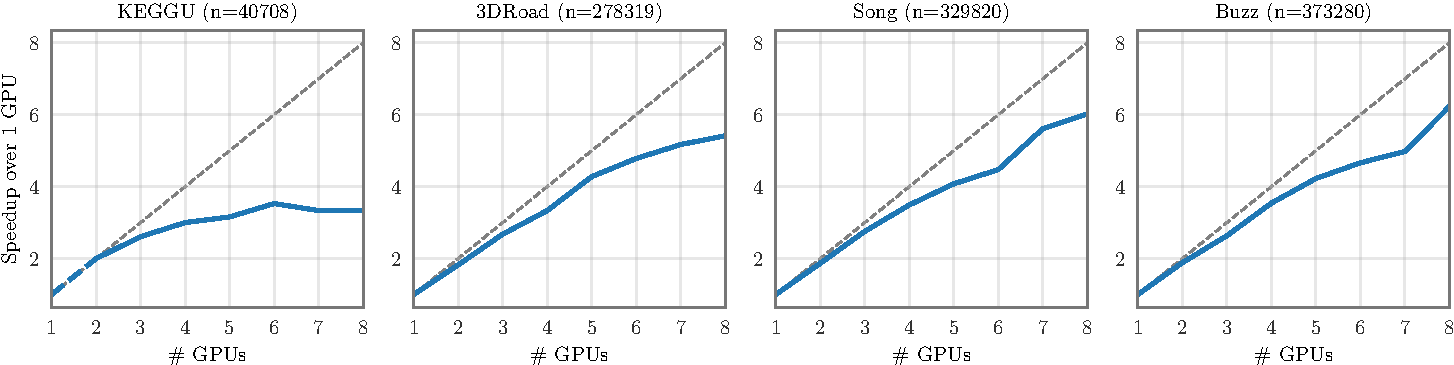
\includegraphics[width=0.70\linewidth]{figures/gpu_speedup.pdf}
  \caption[Speed of BBMM training using multi-GPU computation.]{
    Speed of BBMM training using multi-GPU computation.
    On large datasets, exact GPs with BBMM achieve a near linear speedup with more GPUs.
    (Speedups are measured on NVIDIA Tesla V100-SXM2-32GB-LS GPUs.)
  }
  \label{fig:gpu_speedup}
\end{figure}

\paragraph{Training acceleration with multiple GPUs.}
As discussed in \cref{sec:largeexact_method}, MVMs for training and predictions can be distributed across multiple devices.
\cref{fig:gpu_speedup} plots the speedup as more GPUs are used for training on the KEGGU, 3dRoad, Song, and Buzz datasets.
(Speedups are measured on NVIDIA Tesla V100-SXM2-32GB-LS GPUs without using the KeOps library.)
Each of these datasets achieve a nearly linear speedup up to 4 GPUs.
The speedup is more pronounced for the two large datasets (3dRoad and Song).

\begin{figure*}[t!]
  \centering
  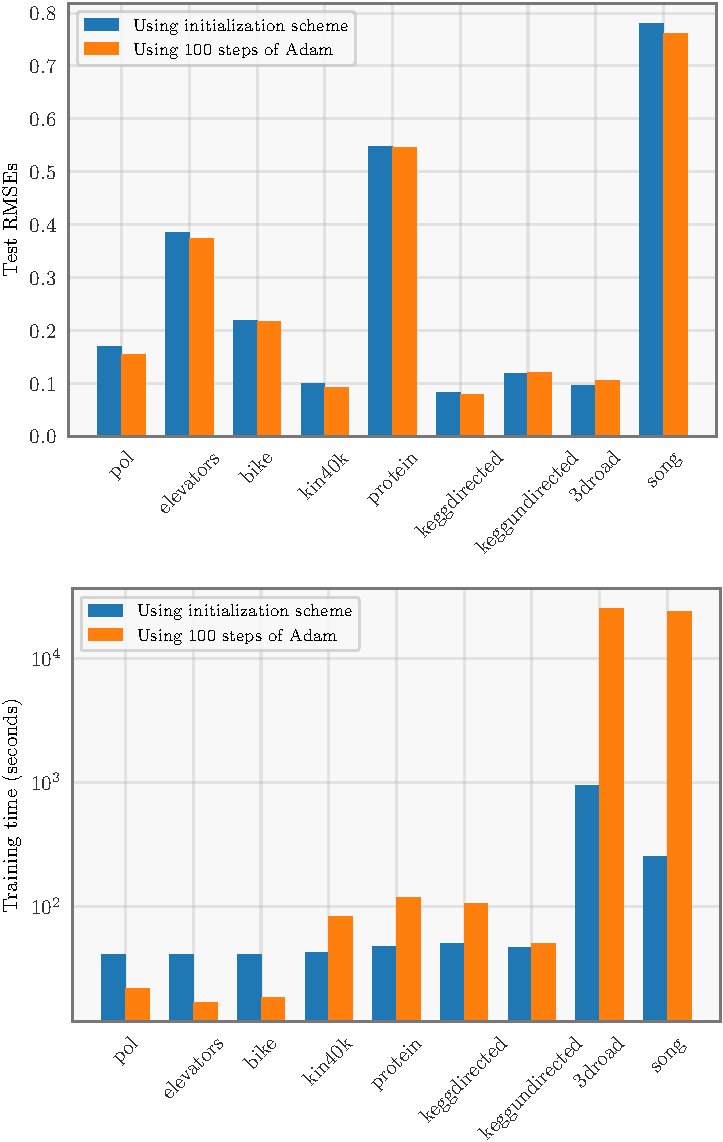
\includegraphics[width=0.75\linewidth]{figures/initialization.pdf}
  \caption[
    Effect of pre-training-based initialization on GP accuracy and timing.
  ]{
    Effect of pre-training-based initialization on GP accuracy and timing.
  }
  \label{fig:initialization}
\end{figure*}

\paragraph{Initialization.}
In \cref{fig:initialization} we compare GP models with and without our pre-training initialization scheme.
The GPs with initialization are pre-trained on a $N=10,\!000$ subset of the training data before running a final $3$ iterations of Adam on the full dataset.
The GPs without initialization are trained on the full dataset for 100 iterations of Adam.
On all datasets, the pre-trained models achieve a comparable test set RMSE as the standard models.
However, the pre-trained models require an \emph{order of magnitude} less training time.
